\documentclass[tikz, border=3mm, convert={outfile=r-type-format-bitfields.png}]{standalone}

\begin{document}

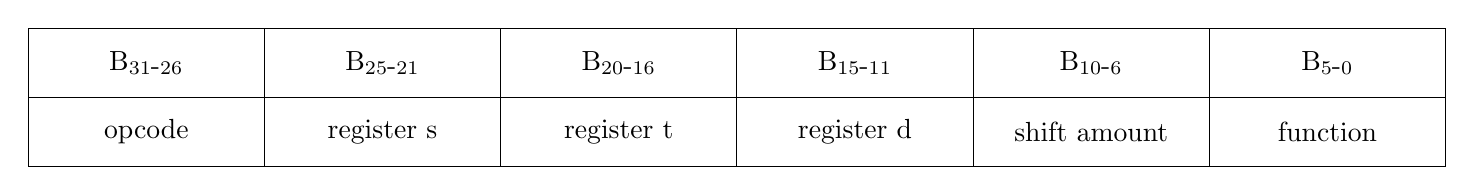
\begin{tikzpicture}[auto,
    every node/.style={inner sep=0pt,rectangle, minimum height=2.5em, text centered, text width=3cm},
    field/.style={draw, text width=3cm, anchor=west}]
\matrix (m) [ampersand replacement=\&, column sep=-\pgflinewidth, row sep=-\pgflinewidth]
{
\node [field] {$\textrm{B}_{31\textrm{-}26}$}; \&
\node [field] {$\textrm{B}_{25\textrm{-}21}$}; \&
\node [field] {$\textrm{B}_{20\textrm{-}16}$}; \&
\node [field] {$\textrm{B}_{15\textrm{-}11}$}; \&
\node [field] {$\textrm{B}_{10\textrm{-}6}$}; \&
\node [field] {$\textrm{B}_{5\textrm{-}0}$}; \&
\\
\node [field] {opcode}; \&
\node [field] {register s}; \&
\node [field] {register t}; \&
\node [field] {register d}; \&
\node [field] {shift amount}; \&
\node [field] {function}; \&
\\
};

\end{tikzpicture}

\end{document}
